\section{Basic Cuda Tasks}

\subsection{Task a}
\begin{figure}[h]
    \begin{center}
        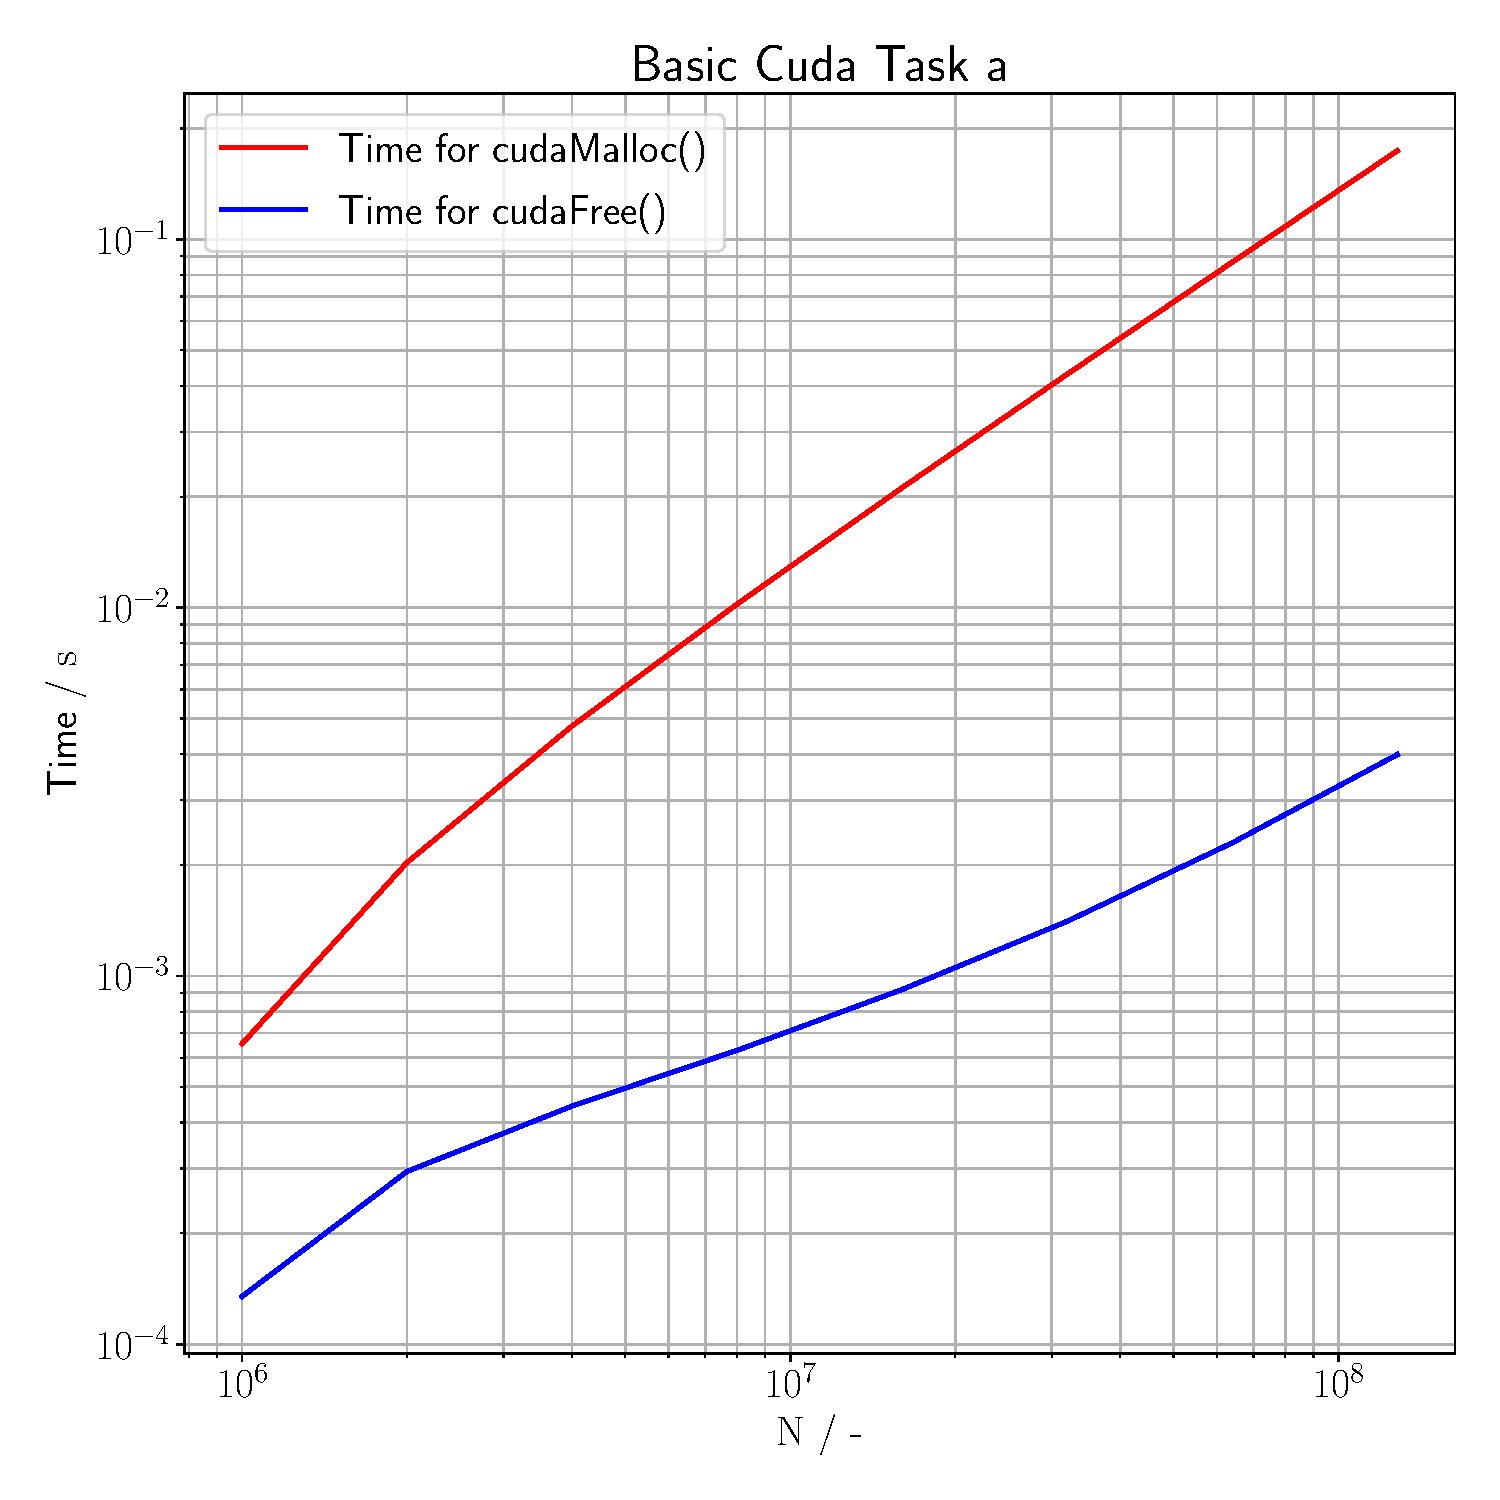
\includegraphics[width=1\textwidth]{figures/task_1_a.pdf}
        \caption{Plot for task 1a - see code in appendix \ref{app_1a}}
        \label{task_1_a_plot}
    \end{center}
\end{figure}
\pagebreak

\subsection{Task b}
\begin{figure}[h]
    \begin{center}
        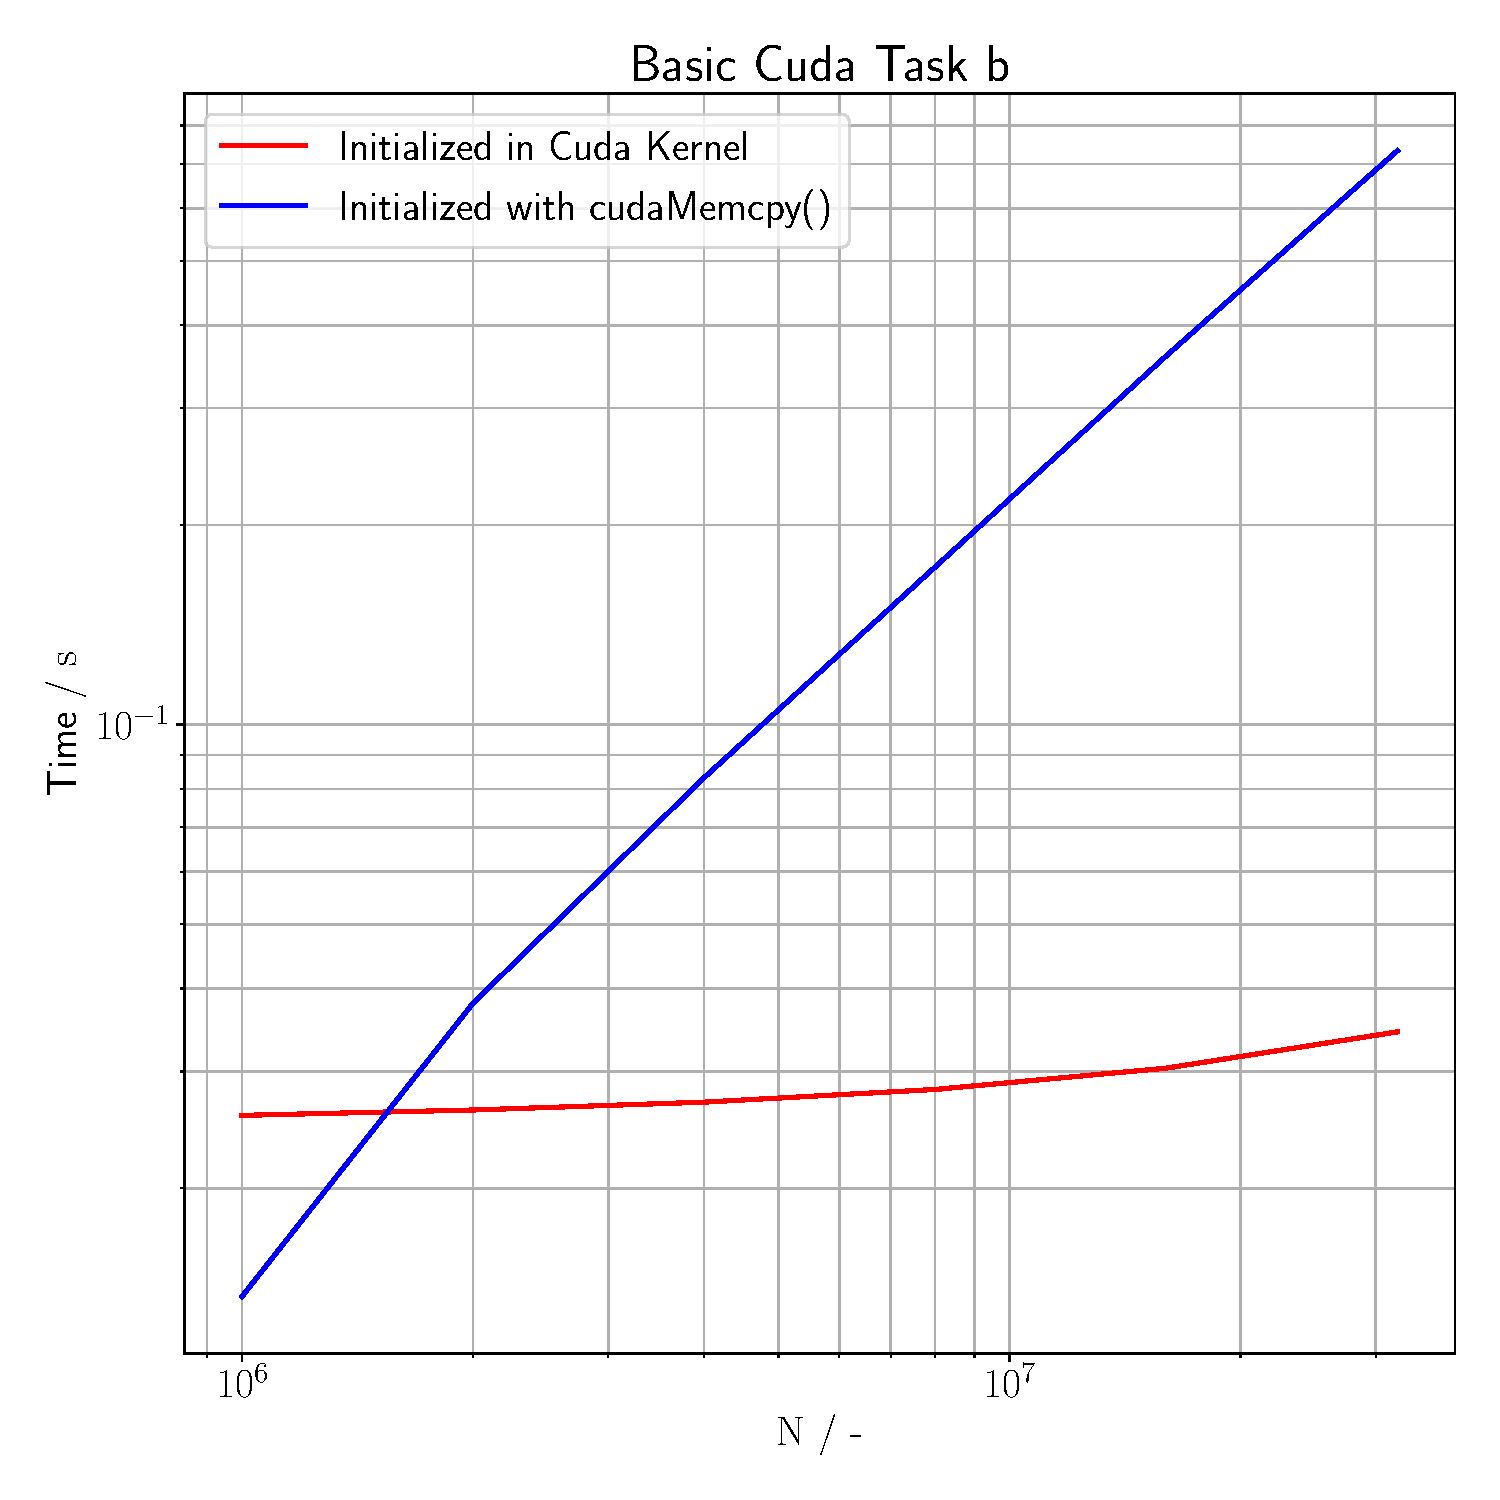
\includegraphics[width=1\textwidth]{figures/task_1_b.pdf}
        \caption{Plot for task 1b - see code in appendix \ref{app_1b}}
        \label{task_1_b_plot}
    \end{center}
\end{figure} 
\pagebreak

\subsection{Task c}
See Implementation in appendix \ref{app_1cde}. \\
\null
\subsection{Task d}
\begin{figure}[h]
    \begin{center}
        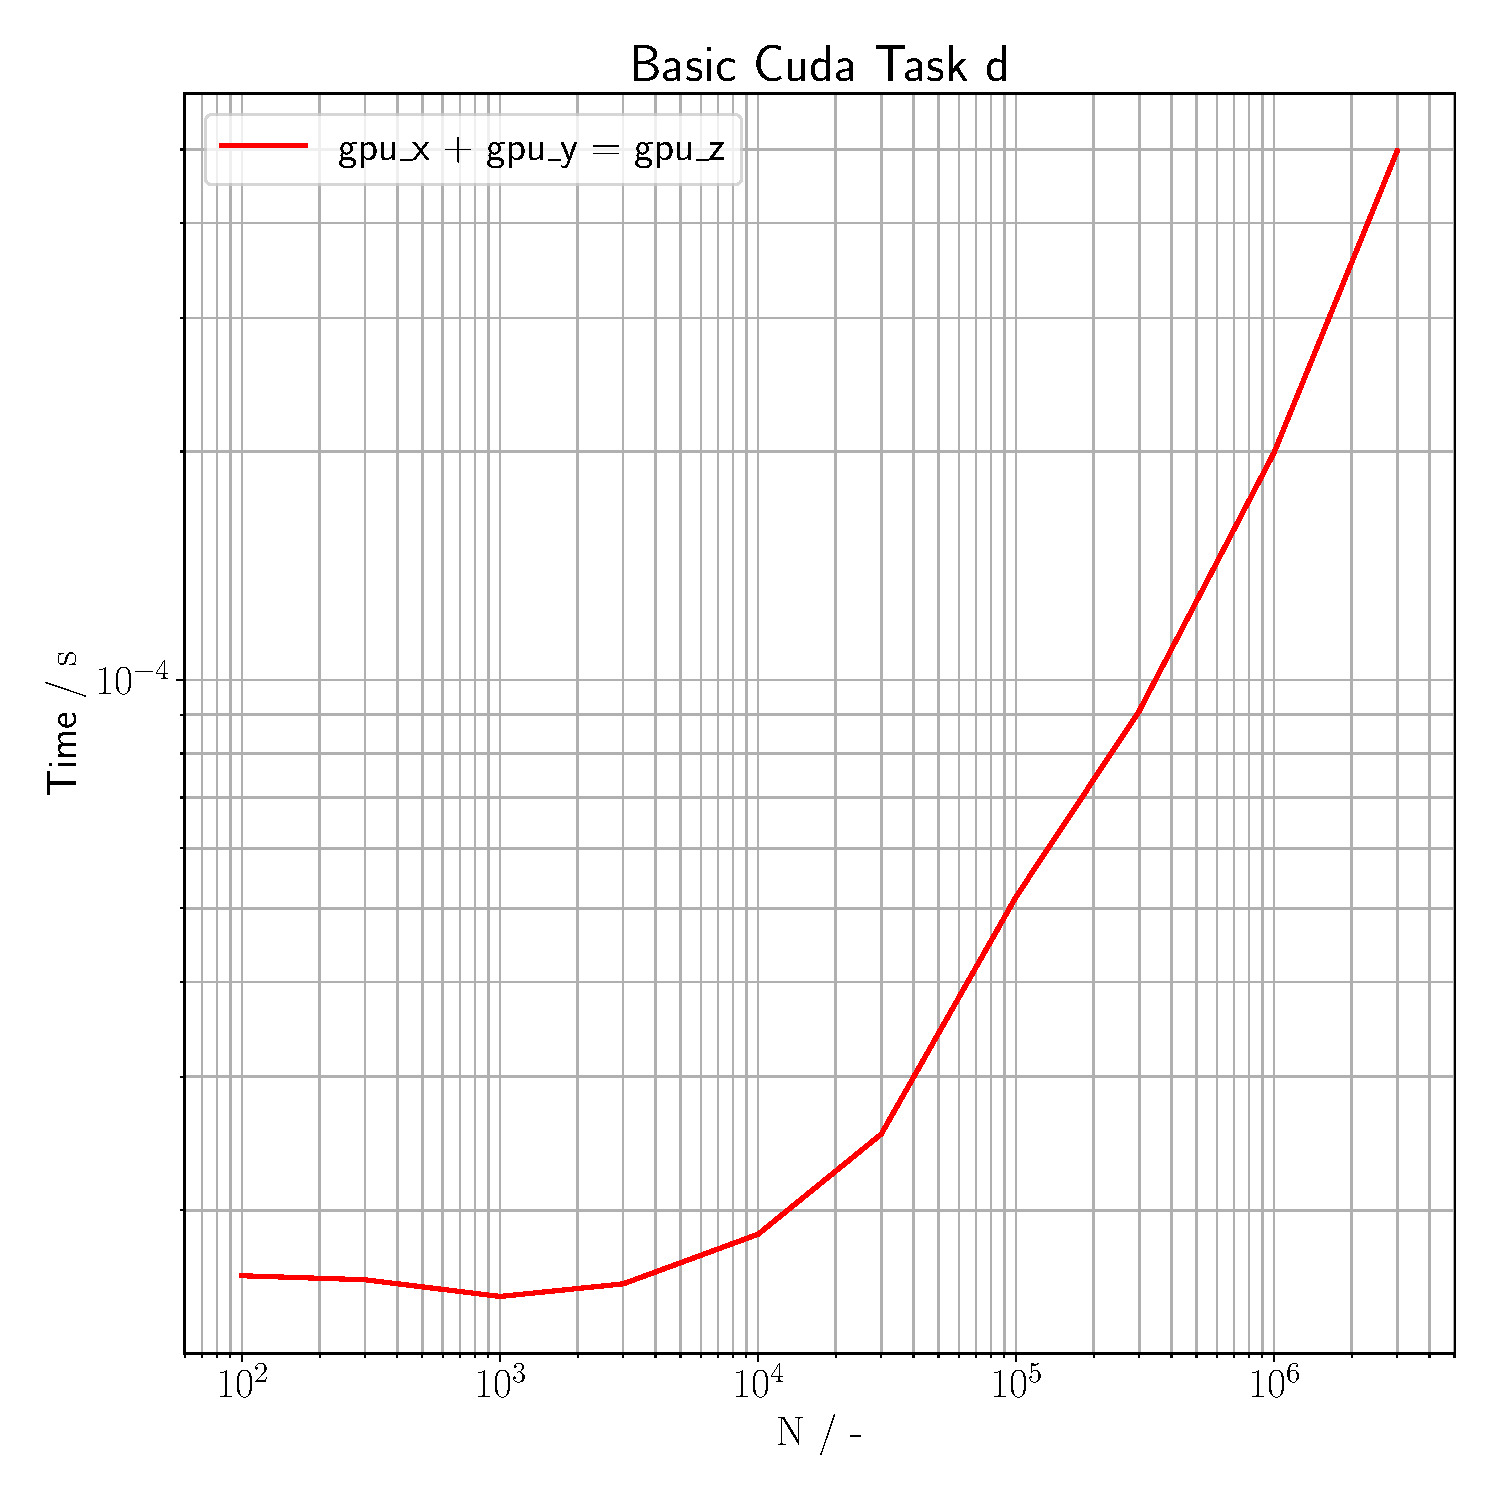
\includegraphics[width=1\textwidth]{figures/task_1_d.pdf}
        \caption{Plot for task 1d - See code in appendix \ref{app_1cde}}
        \label{task_1_d_plot}
    \end{center}
\end{figure}
Until $\mathrm{N}=10^4$, the runtime stays approximately the same, after that, a significant increase
in runtime can be observed.
\pagebreak

\subsection{Task e}
\begin{figure}[h]
    \begin{center}
        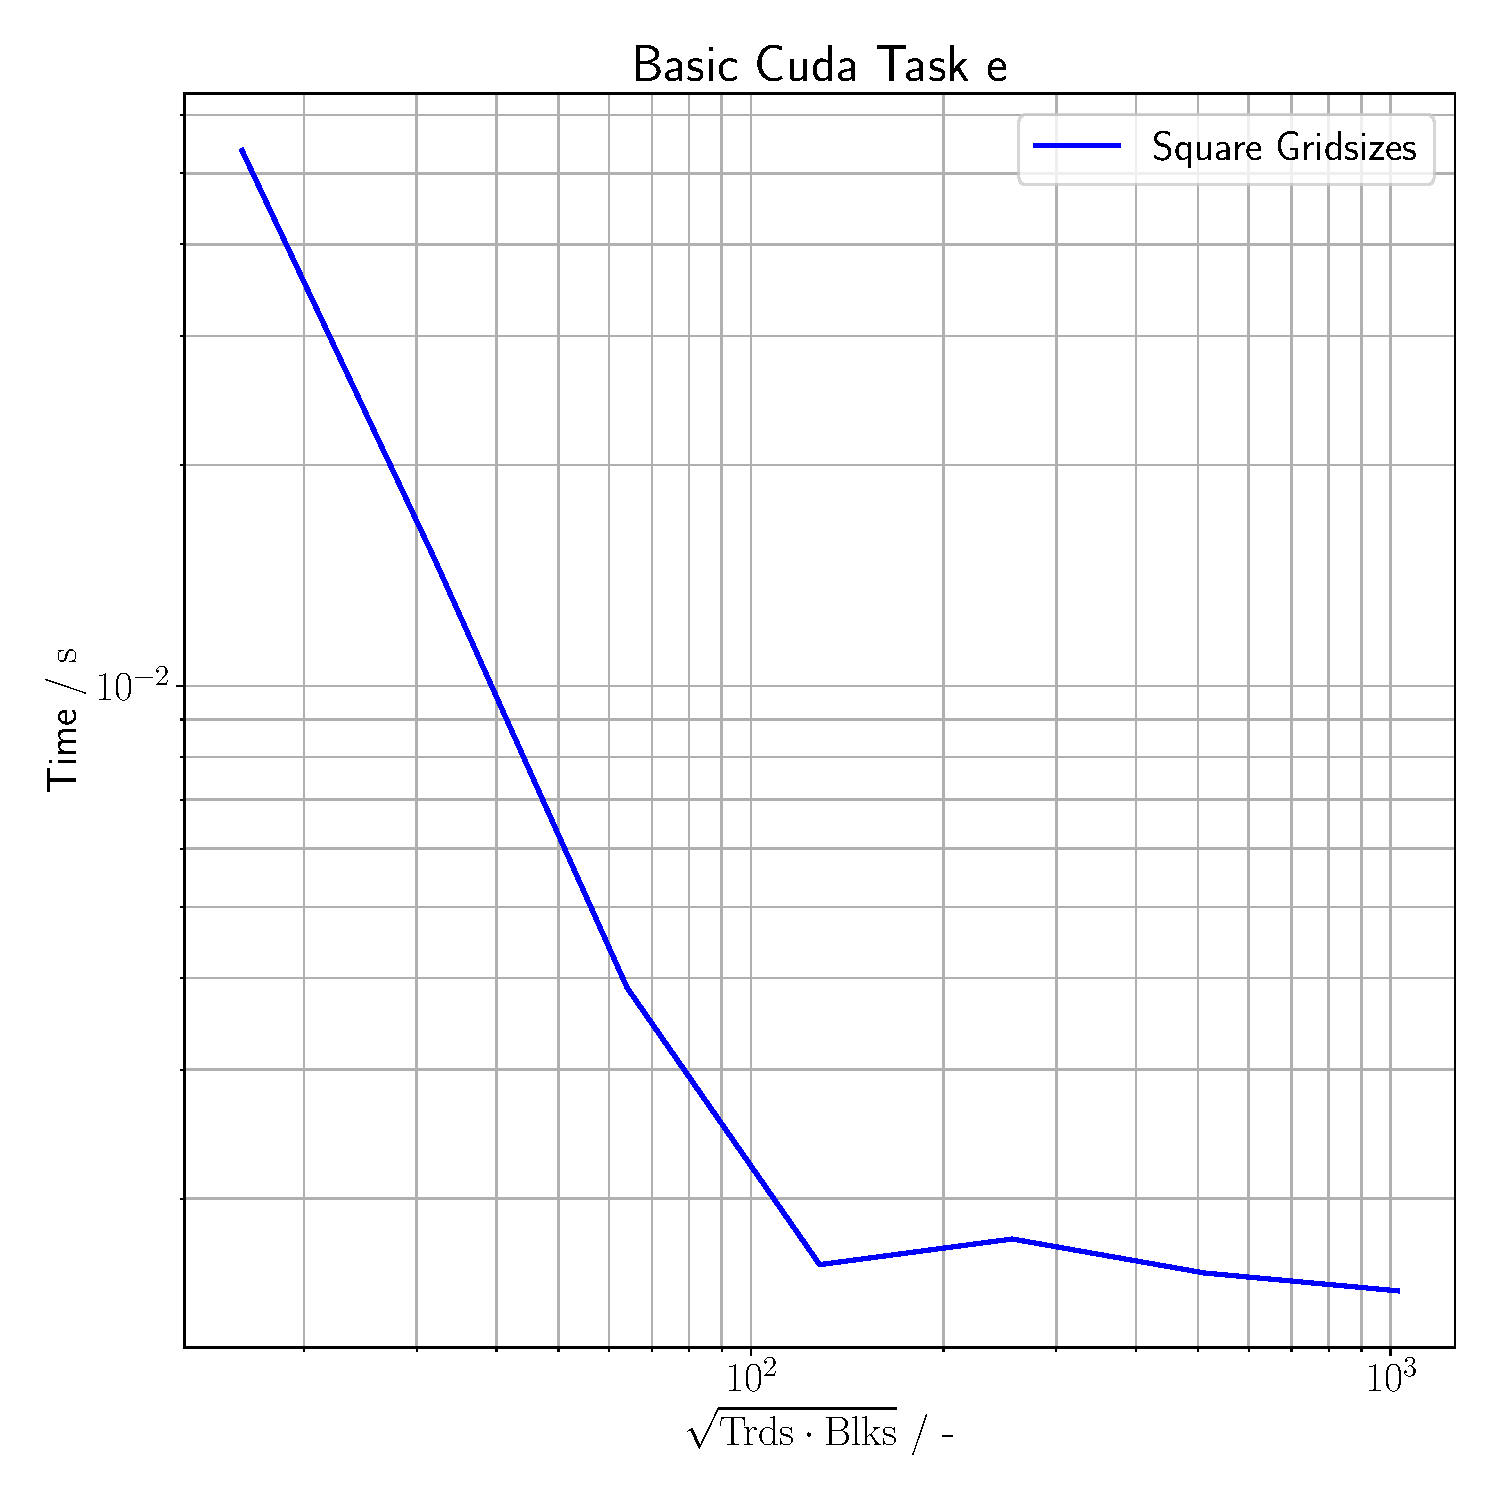
\includegraphics[width=1\textwidth]{figures/task_1_e.pdf}
        \caption{Plot for Task 1e - See code in appendix \ref{app_1cde}}
        \label{task_1_e_plot}
    \end{center}
\end{figure}
For $\sqrt{\mathrm{Trds} \cdot \mathrm{Blks}} < 128 $, there is a signifcant performance decline.
\pagebreak

\section{Dot Product with Cuda}
\subsection{Task a and b}
\begin{figure}[h]
    \begin{center}
        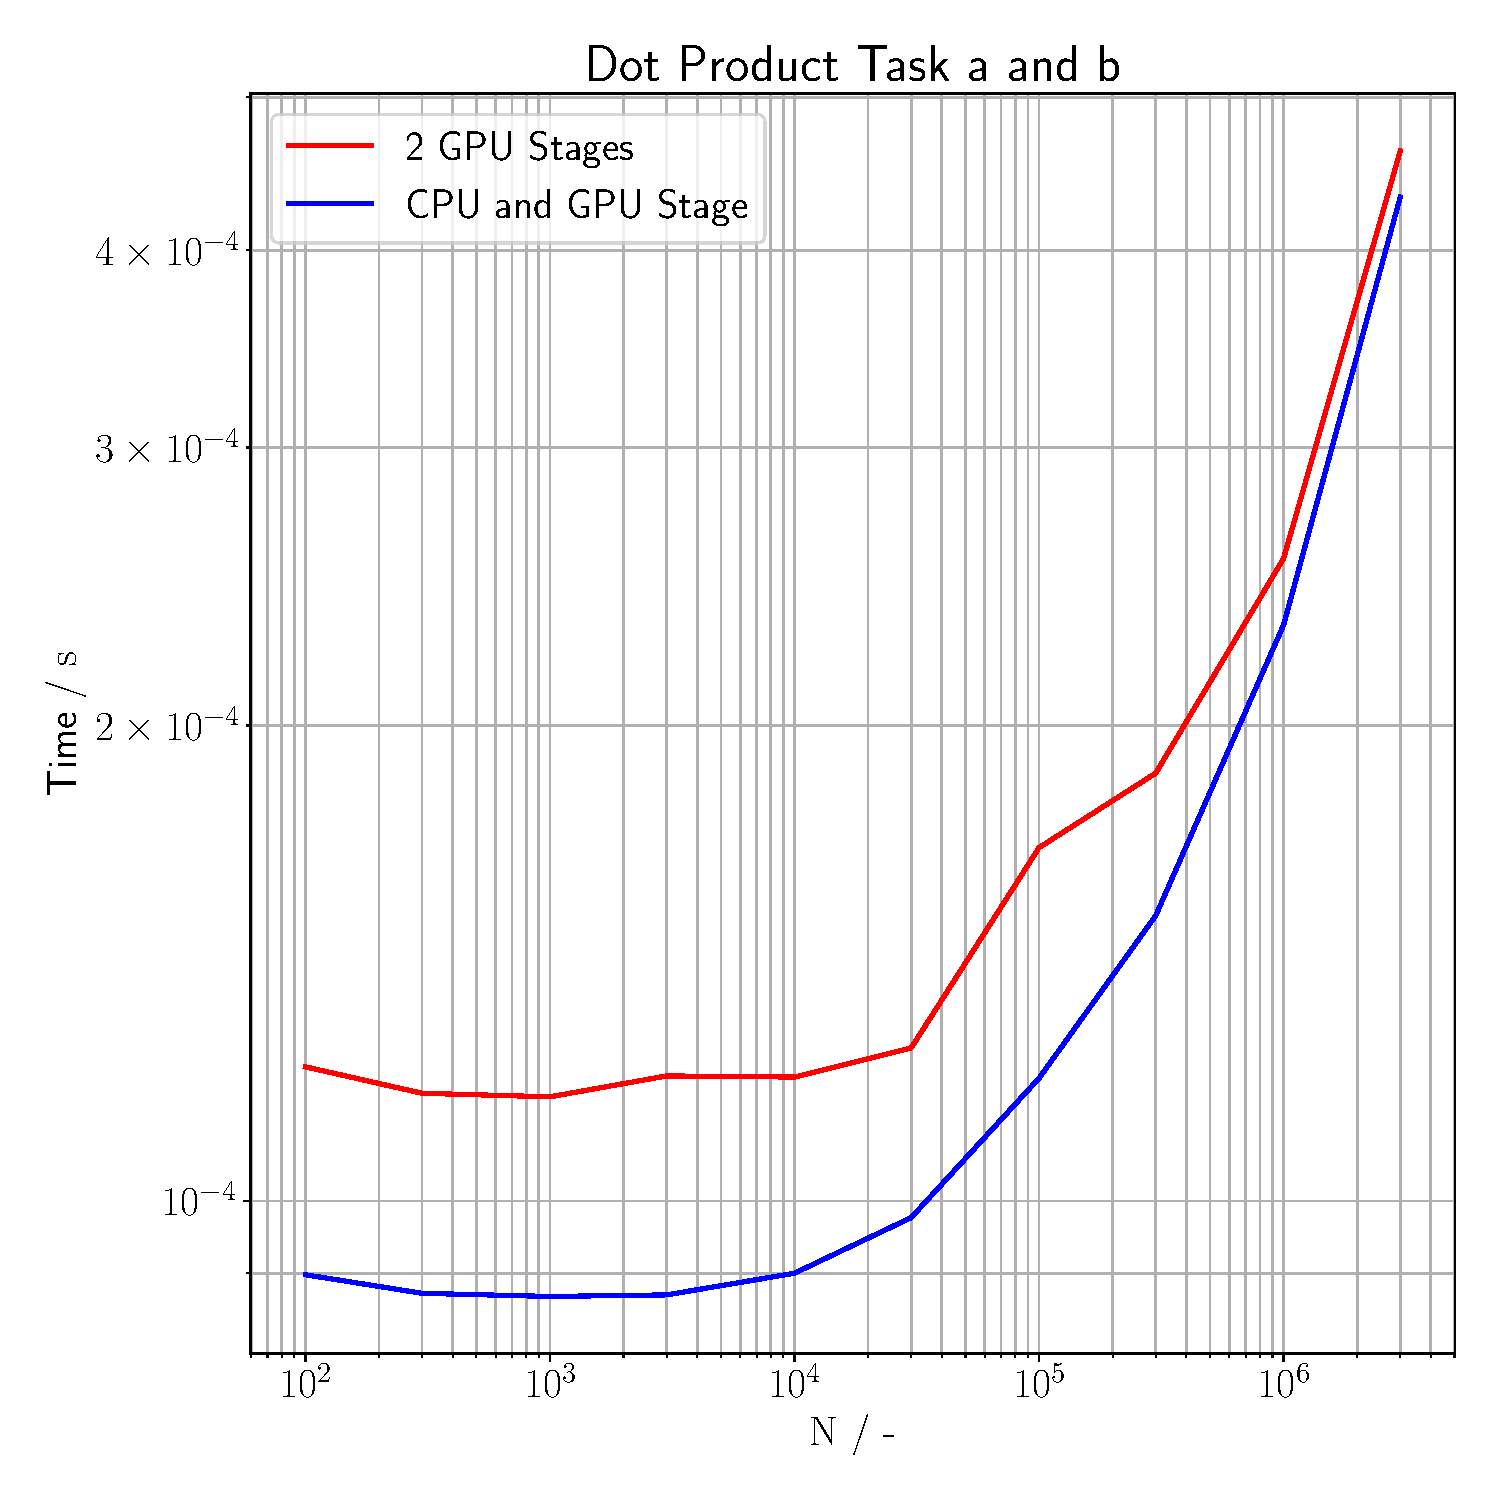
\includegraphics[width=1\textwidth]{figures/dot_product.pdf}
        \caption{Plots for the Dot Product Task - See code in appendix \ref{app_2a} and \ref{app_2b}}
        \label{task_2_ab_plot}
    \end{center}
\end{figure}

Computational tasks which benefit from parallel reduction operations are faster on the given CPU.